% ------------------------------------------------------------------------
% ------------------------------------------------------------------------
% Modelo UFSC para Trabalhos Academicos (tese de doutorado, dissertação de
% mestrado) utilizando a classe abntex2
%
% Autor: Alisson Lopes Furlani
% 	Modificações:
%	- 27/08/2019: Alisson L. Furlani, add pacote 'glossaries' para listas
% - 30/10/2019: Alisson L. Furlani, adjusted some spacing errors and changed math fonts
% - 17/01/2019: Alisson L. Furlani, updated certification page
% - 03/03/2020: Luiz F. P. Droubi, change file to be used as a template with R.
% ------------------------------------------------------------------------
% ------------------------------------------------------------------------
\newlength{\cslhangindent}
\setlength{\cslhangindent}{1.5em}
\newenvironment{CSLReferences}%
  {}%
  {\par}

\documentclass[
	% -- opções da classe memoir --
	12pt,				% tamanho da fonte
	%openright,			% capítulos começam em pág ímpar (insere página vazia caso preciso)
	oneside,			% para impressão no anverso. Oposto a twoside
	a4paper,			% tamanho do papel.
	% -- opções da classe abntex2 --
	chapter=TITLE,		% títulos de capítulos convertidos em letras maiúsculas
	section=TITLE,		% títulos de seções convertidos em letras maiúsculas
	%subsection=TITLE,	% títulos de subseções convertidos em letras maiúsculas
	%subsubsection=TITLE,% títulos de subsubseções convertidos em letras maiúsculas
	% -- opções do pacote babel --
	english,			% idioma adicional para hifenização
	%french,				% idioma adicional para hifenização
	%spanish,			% idioma adicional para hifenização
	brazil				% o último idioma é o principal do documento
	]{abntex2}

\usepackage{setup/ufscthesisA4-alf}

\addbibresource{references.bib}

\usepackage[table]{xcolor}
\let\newfloat\undefined
\usepackage{floatrow}
\floatsetup[table]{capposition=top}
\floatsetup[figure]{capposition=top}

\newcommand{\pkg}[1]{{\normalfont\fontseries{b}\selectfont #1}}
\let\proglang=\textsf
\let\code=\texttt

\usepackage{color}
\usepackage{fancyvrb}
\newcommand{\VerbBar}{|}
\newcommand{\VERB}{\Verb[commandchars=\\\{\}]}
\DefineVerbatimEnvironment{Highlighting}{Verbatim}{commandchars=\\\{\}}
% Add ',fontsize=\small' for more characters per line
\usepackage{framed}
\definecolor{shadecolor}{RGB}{241,243,245}
\newenvironment{Shaded}{\begin{snugshade}}{\end{snugshade}}
\newcommand{\AlertTok}[1]{\textcolor[rgb]{0.68,0.00,0.00}{#1}}
\newcommand{\AnnotationTok}[1]{\textcolor[rgb]{0.37,0.37,0.37}{#1}}
\newcommand{\AttributeTok}[1]{\textcolor[rgb]{0.40,0.45,0.13}{#1}}
\newcommand{\BaseNTok}[1]{\textcolor[rgb]{0.68,0.00,0.00}{#1}}
\newcommand{\BuiltInTok}[1]{\textcolor[rgb]{0.00,0.23,0.31}{#1}}
\newcommand{\CharTok}[1]{\textcolor[rgb]{0.13,0.47,0.30}{#1}}
\newcommand{\CommentTok}[1]{\textcolor[rgb]{0.37,0.37,0.37}{#1}}
\newcommand{\CommentVarTok}[1]{\textcolor[rgb]{0.37,0.37,0.37}{\textit{#1}}}
\newcommand{\ConstantTok}[1]{\textcolor[rgb]{0.56,0.35,0.01}{#1}}
\newcommand{\ControlFlowTok}[1]{\textcolor[rgb]{0.00,0.23,0.31}{#1}}
\newcommand{\DataTypeTok}[1]{\textcolor[rgb]{0.68,0.00,0.00}{#1}}
\newcommand{\DecValTok}[1]{\textcolor[rgb]{0.68,0.00,0.00}{#1}}
\newcommand{\DocumentationTok}[1]{\textcolor[rgb]{0.37,0.37,0.37}{\textit{#1}}}
\newcommand{\ErrorTok}[1]{\textcolor[rgb]{0.68,0.00,0.00}{#1}}
\newcommand{\ExtensionTok}[1]{\textcolor[rgb]{0.00,0.23,0.31}{#1}}
\newcommand{\FloatTok}[1]{\textcolor[rgb]{0.68,0.00,0.00}{#1}}
\newcommand{\FunctionTok}[1]{\textcolor[rgb]{0.28,0.35,0.67}{#1}}
\newcommand{\ImportTok}[1]{\textcolor[rgb]{0.00,0.46,0.62}{#1}}
\newcommand{\InformationTok}[1]{\textcolor[rgb]{0.37,0.37,0.37}{#1}}
\newcommand{\KeywordTok}[1]{\textcolor[rgb]{0.00,0.23,0.31}{#1}}
\newcommand{\NormalTok}[1]{\textcolor[rgb]{0.00,0.23,0.31}{#1}}
\newcommand{\OperatorTok}[1]{\textcolor[rgb]{0.37,0.37,0.37}{#1}}
\newcommand{\OtherTok}[1]{\textcolor[rgb]{0.00,0.23,0.31}{#1}}
\newcommand{\PreprocessorTok}[1]{\textcolor[rgb]{0.68,0.00,0.00}{#1}}
\newcommand{\RegionMarkerTok}[1]{\textcolor[rgb]{0.00,0.23,0.31}{#1}}
\newcommand{\SpecialCharTok}[1]{\textcolor[rgb]{0.37,0.37,0.37}{#1}}
\newcommand{\SpecialStringTok}[1]{\textcolor[rgb]{0.13,0.47,0.30}{#1}}
\newcommand{\StringTok}[1]{\textcolor[rgb]{0.13,0.47,0.30}{#1}}
\newcommand{\VariableTok}[1]{\textcolor[rgb]{0.07,0.07,0.07}{#1}}
\newcommand{\VerbatimStringTok}[1]{\textcolor[rgb]{0.13,0.47,0.30}{#1}}
\newcommand{\WarningTok}[1]{\textcolor[rgb]{0.37,0.37,0.37}{\textit{#1}}}

\newcommand{\bcenter}{\begin{center}}
\newcommand{\ecenter}{\end{center}}

\newcommand{\bapendices}{\begin{apendicesenv}}
\newcommand{\eapendices}{\end{apendicesenv}}

\newcommand{\banexos}{\begin{anexosenv}}
\newcommand{\eanexos}{\end{anexosenv}}

% ---
% Filtering and Mapping Bibliographies
% ---
\DeclareSourcemap{
	\maps[datatype=bibtex]{
		% remove fields that are always useless
		\map{
			\step[fieldset=abstract, null]
			\step[fieldset=pagetotal, null]
		}
		% remove URLs for types that are primarily printed
%		\map{
%			\pernottype{software}
%			\pernottype{online}
%			\pernottype{report}
%			\pernottype{techreport}
%			\pernottype{standard}
%			\pernottype{manual}
%			\pernottype{misc}
%			\step[fieldset=url, null]
%			\step[fieldset=urldate, null]
%		}
		\map{
			\pertype{inproceedings}
			% remove mostly redundant conference information
			\step[fieldset=venue, null]
			\step[fieldset=eventdate, null]
			\step[fieldset=eventtitle, null]
			% do not show ISBN for proceedings
			\step[fieldset=isbn, null]
			% Citavi bug
			\step[fieldset=volume, null]
		}
	}
}
% ---

% ---
% Informações de dados para CAPA e FOLHA DE ROSTO
% ---
% FIXME Substituir 'Nome completo do autor' pelo seu nome.
\autor{Jane Doe}
% FIXME Substituir 'Título do trabalho' pelo título da trabalho.
\titulo{Template Quarto Book}
% FIXME Substituir 'Subtítulo (se houver)' pelo subtítulo da trabalho.
% Caso não tenha substítulo, comente a linha a seguir.
  \subtitulo{SUBTÍTULO}
% FIXME Substituir 'XXXXXX' pelo nome do seu
% orientador.
\orientador{Mauricio Uriona Maldonado}
% FIXME Se for orientado por uma mulher, comente a linha acima e descomente a linha a seguir.
% \orientador[Orientadora]{Nome da orientadora, Dra.}
% FIXME Substituir 'XXXXXX' pelo nome do seu
% coorientador. Caso não tenha coorientador, comente a linha a seguir.
% FIXME Se for coorientado por uma mulher, comente a linha acima e descomente a linha a seguir.
% \coorientador[Coorientadora]{XXXXXX, Dra.}
% FIXME Substituir '[ano]' pelo ano (ano) em que seu trabalho foi defendido.
\ano{\texttt{r\ lubridate::year(Sys.time())}}
% FIXME Substituir '[dia] de [mês] de [ano]' pela data em que ocorreu sua defesa.
\data{31 de Março de \texttt{r\ lubridate::year(Sys.time())}}
% FIXME Substituir 'Local' pela cidade em que ocorreu sua defesa.
\local{Florianópolis}
\instituicaosigla{UFSC}
\instituicao{Universidade Federal de Santa Catarina}
% FIXME Substituir 'Dissertação/Tese' pelo tipo de trabalho (Tese, Dissertação).
\tipotrabalho{Trabalho de Conclusão de Curso}
% FIXME Substituir '[mestre/doutor] em XXXXXX' pela grau adequado.
\formacao{Graduado em Engenharia de Produção Mecânica/Elétrica/Civil}
% FIXME Substituir '[mestrado/doutorado]' pelo nivel adequado.
\nivel{graduação}
% FIXME Substituir 'Programa de Pós-Graduação em XXXXXX' pela curso adequado.
\programa{Departamento de Engenharia de Produção e Sistemas}
% FIXME Substituir 'Campus XXXXXX ou Centro de XXXXXX' pelo campus ou centro adequado.
\centro{CTC - CENTRO TECNOLÓGICO}
\preambulo
{%
\imprimirtipotrabalho~submetida~ao~\imprimirprograma~da~\imprimirinstituicao~para~a~obtenção~do~título~de~\imprimirformacao.
}
% ---

% ---
% Configurações de aparência do PDF final
% ---
% alterando o aspecto da cor azul
\definecolor{blue}{RGB}{41,5,195}
% informações do PDF
\makeatletter
\hypersetup{
     	%pagebackref=true,
		pdftitle={\@title},
		pdfauthor={\@author},
    	pdfsubject={\imprimirpreambulo},
	    pdfcreator={LaTeX with abnTeX2},
		pdfkeywords={ufsc, latex, abntex2},
		colorlinks=true,       		% false: boxed links; true: colored links
    	linkcolor=black,%blue,          	% color of internal links
    	citecolor=black,%blue,        		% color of links to bibliography
    	filecolor=black,%magenta,      		% color of file links
		urlcolor=black,%blue,
		bookmarksdepth=4
}
\makeatother
% ---

% ---
% compila a lista de abreviaturas e siglas e a lista de símbolos
% ---

% Declaração das siglas
\siglalista{ABNT}{Associação Brasileira de Normas Técnicas}
\siglalista{Bacen}{Banco Central do Brasil}


% Declaração dos simbolos
\simbololista{C}{\ensuremath{C}}{Circunferência de um círculo}
\simbololista{pi}{\ensuremath{\pi}}{Número pi}
\simbololista{r}{\ensuremath{r}}{Raio de um círculo}
\simbololista{A}{\ensuremath{A}}{Área de um círculo}


% compila a lista de abreviaturas e siglas e a lista de símbolos
\makenoidxglossaries

% ---

% ---
% compila o indice
% ---
\makeindex
% ---

% ----
% Início do documento
% ----
\begin{document}

% Seleciona o idioma do documento (conforme pacotes do babel)
%\selectlanguage{english}
\selectlanguage{brazil}

% Retira espaço extra obsoleto entre as frases.
\frenchspacing

% Espaçamento 1.5 entre linhas
\OnehalfSpacing

% Corrige justificação
%\sloppy

% ----------------------------------------------------------
% ELEMENTOS PRÉ-TEXTUAIS
% ----------------------------------------------------------
% \pretextual %a macro \pretextual é acionado automaticamente no início de \begin{document}
% ---
% Capa, folha de rosto, ficha bibliografica, errata, folha de apróvação
% Dedicatória, agradecimentos, epígrafe, resumos, listas
% ---
% ---
% Capa
% ---
\imprimircapa
% ---

% ---
% Folha de rosto
% (o * indica que haverá a ficha bibliográfica)
% ---
\imprimirfolhaderosto*
% ---

% ---
% Inserir a ficha bibliografica
% ---
% http://ficha.bu.ufsc.br/
\begin{fichacatalografica}
	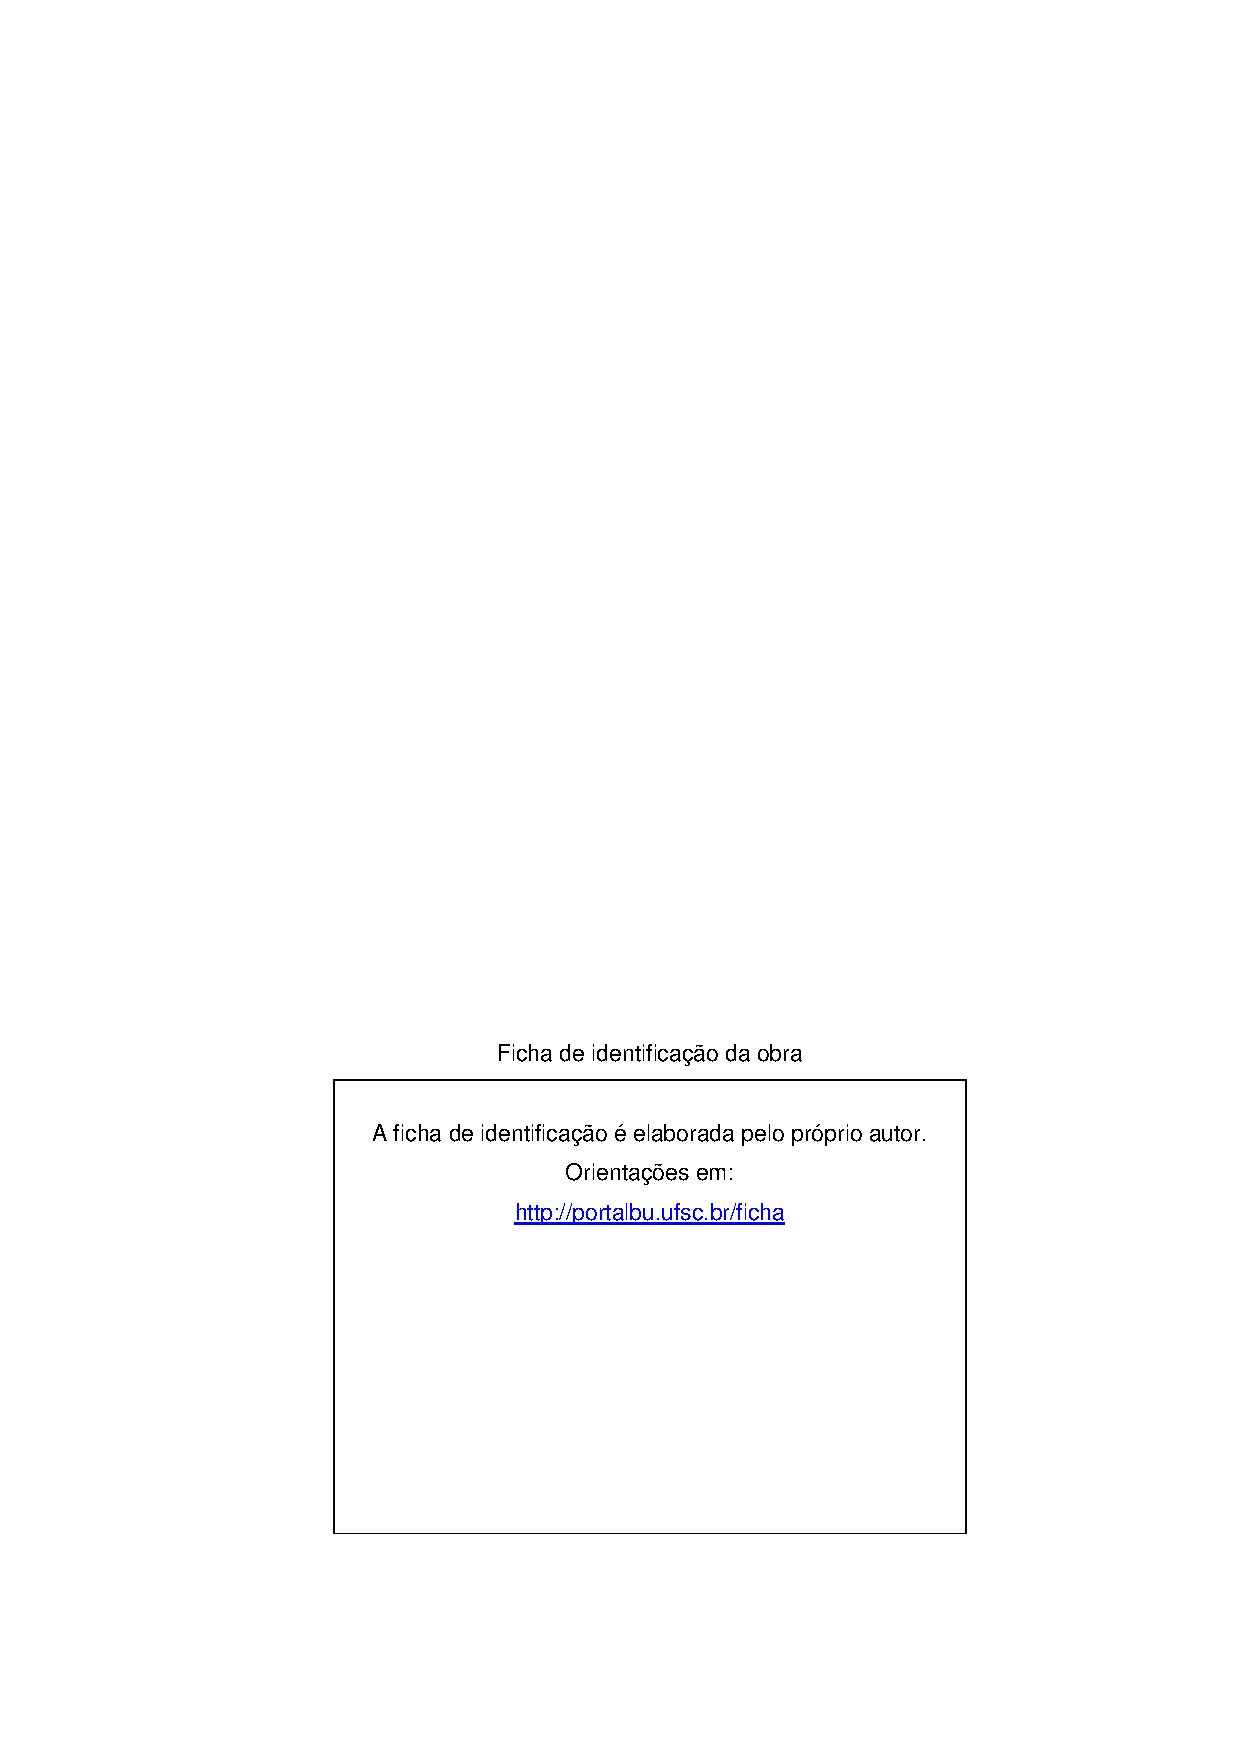
\includepdf{Ficha_Catalografica.pdf}
\end{fichacatalografica}
% ---

% ---
% Inserir folha de aprovação
% ---
\begin{folhadeaprovacao}
	\OnehalfSpacing
	\centering
	\imprimirautor\\%
	\vspace*{10pt}		
	\textbf{\imprimirtitulo}%
	\ifnotempty{\imprimirsubtitulo}{:~\imprimirsubtitulo}\\%
	%		\vspace*{31.5pt}%3\baselineskip
	\vspace*{\baselineskip}
	%\begin{minipage}{\textwidth}
	O presente trabalho em nível de \imprimirnivel~foi avaliado e aprovado por banca examinadora composta pelos seguintes membros:\\
	%\end{minipage}%
	\vspace*{\baselineskip}
    Prof. Examinador 1, Dr.\\
  Universidade Federal de Santa Catarina - UFSC\\
  \vspace*{\baselineskip}
    Prof. Examinador 2, Dr.\\
  Fédération Internationale des Géomètres - FIG\\
  \vspace*{\baselineskip}
    
	\vspace*{2\baselineskip}
	\begin{minipage}{\textwidth}
		Certificamos que esta é a \textbf{versão original e final} do trabalho de conclusão que foi julgado adequado para obtenção do título de \imprimirformacao.\\
	\end{minipage}
	%    \vspace{-0.7cm}
	\vspace*{\fill}
	\assinatura{\OnehalfSpacing Beltrano da
Silva \\ Coordenação do Programa de Pós-Graduação}
	\vspace*{\fill}
	\assinatura{\OnehalfSpacing\imprimirorientador \\ \imprimirorientadorRotulo}
	%	\ifnotempty{\imprimircoorientador}{
	%	\assinatura{\imprimircoorientador \\ \imprimircoorientadorRotulo \\
	%		\imprimirinstituicao~--~\imprimirinstituicaosigla}
	%	}
	% \newpage
	\vspace*{\fill}
	\imprimirlocal, \imprimirano.
\end{folhadeaprovacao}
% ---

% ---
% Dedicatória
% ---
\begin{dedicatoria}
	\vspace*{\fill}
	\noindent
	\begin{adjustwidth*}{}{5.5cm} 
		\raggedleft       
		Este trabalho é dedicado aos meus colegas de classe e aos meus queridos
pais.
	\end{adjustwidth*}
\end{dedicatoria}
% ---

% ---
% Agradecimentos
% ---
\begin{agradecimentos}
	Gostaria de agradecer sinceramente a todos os que colaboraram à
execução\\
deste trabalho.\\
Aos colegas da UFSC.\\
Aos professores do PPGTG.\\
Em especial ao meu orientador, pela paciência.\\
E a minha querida esposa pela compreensão.
\end{agradecimentos}
% ---

% ---
% Epígrafe
% ---
\begin{epigrafe}
	\vspace*{\fill}
	\begin{flushright}
		\textit{``Eppur si muove!''\\
(Galileu Galilei, 1633)}
	\end{flushright}
\end{epigrafe}
% ---

% ---
% RESUMOS
% ---

% resumo em português
\setlength{\absparsep}{18pt} % ajusta o espaçamento dos parágrafos do resumo
\begin{resumo}
	\SingleSpacing
  No resumo são ressaltados o objetivo da pesquisa, o método utilizado,
as discussões e os resultados com destaque apenas para os pontos
principais. O resumo deve ser significativo, composto de uma sequência
de frases concisas, afirmativas, e não de uma enumeração de tópicos. Não
deve conter citações. Deve usar o verbo na voz ativa e na terceira
pessoa do singular. O texto do resumo deve ser digitado, em um único
bloco, sem espaço de parágrafo. O espaçamento entre linhas é simples e o
tamanho da fonte é 12. Abaixo do resumo, informar as palavras-chave
(palavras ou expressões significativas retiradas do texto) ou, termos
retirados de thesaurus da área. Deve conter de 150 a 500 palavras. O
resumo é elaborado de acordo com a NBR 6028. 
  
  \textbf{Palavras-chave}: 
    Palavra-chave 1.
    Palavra-chave 2.
  \end{resumo}

% resumo em inglês
\begin{resumo}[Abstract]
	\SingleSpacing
	\begin{otherlanguage*}{english}
		Resumo traduzido para outros idiomas, neste caso, inglês. Segue o
formato do resumo feito na língua vernácula. As palavras-chave
traduzidas, versão em língua estrangeira, são colocadas abaixo do texto
precedidas pela expressão Keywords, separadas por ponto.
		
		\textbf{Keywords}:
	      Keyword 1.
        Keyword 2.
    	\end{otherlanguage*}
\end{resumo}

%% resumo em francês 
%\begin{resumo}[Résumé]
% \begin{otherlanguage*}{french}
%    Il s'agit d'un résumé en français.
% 
%   \textbf{Mots-clés}: latex. abntex. publication de textes.
% \end{otherlanguage*}
%\end{resumo}
%
%% resumo em espanhol
%\begin{resumo}[Resumen]
% \begin{otherlanguage*}{spanish}
%   Este es el resumen en español.
%  
%   \textbf{Palabras clave}: latex. abntex. publicación de textos.
% \end{otherlanguage*}
%\end{resumo}
%% ---

{%hidelinks
	\hypersetup{hidelinks}
	% ---
	% inserir lista de ilustrações
	% ---
	\pdfbookmark[0]{\listfigurename}{lof}
	\listoffigures*
	\cleardoublepage
	% ---
	
	% ---
	% inserir lista de quadros
	% ---
	\pdfbookmark[0]{\listofquadrosname}{loq}
	\listofquadros*
	\cleardoublepage
	% ---
	
	% ---
	% inserir lista de tabelas
	% ---
	\pdfbookmark[0]{\listtablename}{lot}
	\listoftables*
	\cleardoublepage
	% ---
	
	% ---
	% inserir lista de abreviaturas e siglas (devem ser declarados no preambulo)
	% ---
	\imprimirlistadesiglas
	% ---
	
	% ---
	% inserir lista de símbolos (devem ser declarados no preambulo)
	% ---
	\imprimirlistadesimbolos
	% ---
	
	% ---
	% inserir o sumario
	% ---
	\pdfbookmark[0]{\contentsname}{toc}
	\tableofcontents*
	\cleardoublepage
	
}%hidelinks
% ---

% ---

% ----------------------------------------------------------
% ELEMENTOS TEXTUAIS
% ----------------------------------------------------------

\phantompart

\textual

\bookmarksetup{startatroot}

\hypertarget{section}{%
\chapter*{}\label{section}}
\addcontentsline{toc}{chapter}{}

\bookmarksetup{startatroot}

\hypertarget{intro}{%
\chapter{Introdução}\label{intro}}

As orientações aqui apresentadas são baseadas em um conjunto de normas
elaboradas pela \gls{ABNT}. Além das normas técnicas, a Biblioteca
também elaborou uma série de tutoriais, guias, \emph{templates} os quais
estão disponíveis em seu site, no endereço
\url{http://portal.bu.ufsc.br/normalizacao/}.

Paralelamente ao uso deste \emph{template} recomenda-se que seja
utilizado o \textbf{Tutorial de Trabalhos Acadêmicos} (disponível neste
\href{/url\%7Bhttps://repositorio.ufsc.br/handle/123456789/180829}{link})
e/ou que o discente \textbf{participe das capacitações oferecidas da
Biblioteca Universitária da UFSC}.

Este \emph{template} está configurado apenas para a impressão utilizando
o anverso das folhas, caso você queira imprimir usando a frente e o
verso, acrescente a opção \emph{openright} e mude de \emph{oneside} para
\emph{twoside} nas configurações da classe \emph{abntex2} no início do
arquivo principal \emph{main.tex}
(\protect\hyperlink{ref-abntex2classe}{ARAUJO, 2015}).

Conforme a
\href{https://repositorio.ufsc.br/bitstream/handle/123456789/197121/RN46.2019.pdf?sequence=1\&isAllowed=y}{Resolução
NORMATIVA nº 46/2019/CPG} as dissertações e teses não serão mais
entregues em formato impresso na Biblioteca Universitária. Consulte o
Repositório Institucional da UFSC ou sua Secretaria de Pós Graduação
sobre os procedimentos para a entrega
(\protect\hyperlink{ref-anfavea2006}{ANFAVEA, 2006}).

\hypertarget{objetivos}{%
\section{Objetivos}\label{objetivos}}

Nas seções abaixo estão descritos o objetivo geral e os objetivos
específicos.

\hypertarget{objetivo-geral}{%
\subsection{Objetivo Geral}\label{objetivo-geral}}

Descrição\ldots{}\gls{Bacen}

\hypertarget{objetivos-especuxedficos}{%
\subsection{Objetivos Específicos}\label{objetivos-especuxedficos}}

Descrição\ldots{}

\bookmarksetup{startatroot}

\hypertarget{introduction}{%
\chapter{Introduction}\label{introduction}}

This is a book created from markdown and executable code.

See KNUTH (\protect\hyperlink{ref-knuth84}{1984}) for additional
discussion of literate programming.

\begin{Shaded}
\begin{Highlighting}[]
\DecValTok{1} \SpecialCharTok{+} \DecValTok{1}
\end{Highlighting}
\end{Shaded}

\begin{verbatim}
[1] 2
\end{verbatim}

\bookmarksetup{startatroot}

\hypertarget{summary}{%
\chapter{Summary}\label{summary}}

In summary, this book has no content whatsoever.

\begin{Shaded}
\begin{Highlighting}[]
\DecValTok{1} \SpecialCharTok{+} \DecValTok{1}
\end{Highlighting}
\end{Shaded}

\begin{verbatim}
[1] 2
\end{verbatim}

\bookmarksetup{startatroot}

\hypertarget{referuxeancias}{%
\chapter*{Referências}\label{referuxeancias}}
\addcontentsline{toc}{chapter}{Referências}

\hypertarget{refs}{}
\begin{CSLReferences}{0}{1}
\leavevmode\vadjust pre{\hypertarget{ref-anfavea2006}{}}%
ANFAVEA. \emph{Indústria automobilística brasileira}. {[}S.l: s.n.{]},
2006.

\leavevmode\vadjust pre{\hypertarget{ref-abntex2classe}{}}%
ARAUJO, L. C. \emph{A classe abntex2: Modelo canônico de trabalhos
acadêmicos brasileiros compatível com as normas ABNT NBR 14724:2011,
ABNT NBR 6024:2012 e outras}. {[}S.l.{]}: Equipe abnTeX2, 2015.
Disponível em: \textless{}\url{http://www.abntex.net.br/}\textgreater.
Acesso em: 16 ago. 2019.

\leavevmode\vadjust pre{\hypertarget{ref-knuth84}{}}%
KNUTH, D. E. Literate Programming. \emph{Comput. J.}, v. 27, n. 2, p.
97--111, 1984. Disponível em:
\textless{}\url{https://doi.org/10.1093/comjnl/27.2.97}\textgreater.

\end{CSLReferences}

% ----------------------------------------------------------
% Glossário
% ----------------------------------------------------------
%
% Consulte o manual da classe abntex2 para orientações sobre o glossário.
%
%\glossary

%---------------------------------------------------------------------
% INDICE REMISSIVO
%---------------------------------------------------------------------
%\phantompart
%\printindex
%---------------------------------------------------------------------

\end{document}
